% !TEX root =  ./main.tex

\subsection{Protein Signaling Networks Analysis}\label{sec:ccReact}
\textcolor{red}{Check if the studies were also present in: Artur Meski, Wojciech Penczek, Grzegorz Rozenberg: Model checking
temporal properties of reaction systems. Inf. Sci. 313: 22-42 (2015)}
This case was studied in~\cite{DBLP:conf/cmsb/BallisBFO24}, where it was encoded into the Maude\footnote{\url{https://maude.cs.illinois.edu}.} ecosystem~\cite{DBLP:conf/maude/2007} to take advantage of their built-in LTL and CTL model checker facilities. It is based on a biological case study from~\cite{derHeyde2014}, aimed to identify the best drug treatment for three different breast cancer representative cell lines: BT474, SKBR3 and HCC1954. This is achieved by studying the behavior of the protein signaling networks for the HER2-positive breast cancer subtype in the presence of different combinations of monoclonal antibody drugs.
%The paper~\cite{DBLP:conf/cmsb/BallisBFO24} encodes RSs into the Maude ecosystem\footnote{\url{https://maude.cs.illinois.edu}.}~\cite{DBLP:conf/maude/2007} to take advantage of the built-in LTL and CTL model checker facilities.
In a nutshell, Maude is a high-performance reflective language and system based on equational and rewriting logic specification. 
The encoding of RSs is made possible by setting up a specific rewrite theory, called \textbf{ccReact}, which is expressive enough to capture the relevant aspects of the protein signaling networks.
%incorporate reactions and guarded contexts.
%The approach is then validated on a biological case study taken from~\cite{derHeyde2014}, aimed to identify the best drug treatment for three different breast cancer representative cell lines: BT474, SKBR3 and HCC1954. This is achieved by studying the behavior of the protein signaling networks for the HER2-positive breast cancer subtype in the presence of different combinations of monoclonal antibody drugs.
The analysis conducted in~\cite{DBLP:conf/cmsb/BallisBFO24} matches previous findings, and makes it possible to readily inspect new hypotheses.

\subparagraph*{Analysis goals.}
The goal of the analysis is to exploit model checking to validate or refute some behavioural hypotheses of RSs.

\subparagraph*{Features of interest.}
Besides reachability analysis, mostly concerned with the possibility to reach certain attractors, the distinguishing feature of this case study is the possibility to model check RSs with guarded contexts against behavioural properties written in LTL and CTL.

\subparagraph*{Experimental set up.}
The technique in~\cite{DBLP:conf/cmsb/BallisBFO24} starts directly from a RS specification, which is manually coded in \textbf{ccReact} and queried using Maude state exploration techniques and built-in model checkers. Likewise, here we can just exploit the direct translation of RSs (with guarded contexts) to \GROOVE presented in the previous section, i.e., no preprocessing is necessary. The \BioResolve specification is in \Cref{fig:bioresolve:psn} in \Cref{app:psn}.
The following properties have been experimented with:
\begin{enumerate}
\item searching for the the presence/absence of the attractor \texttt{akt} in steady states of the BT747 cell line,\todo{Is this really about steady states? The LTL formula on page 14, line 4 of the paper specifies \texttt{io-state}, not \texttt{isSteady}.} where the context \verb=[k,ket]= is considered;

\item in order to observe the interactions when either \texttt{e}rlotinib or \texttt{p}ertuzumab are supplied, the context \verb=[{e,egf,hrg}.korep]= is considered and Maude reports that there exists at least one path where that treatment is successful, but not all paths avoid a steady state where \texttt{akt} is present;

\item using the context \verb=[k,korept]=, it is shown that, regardless the drug used, once \texttt{pdk1} is present, inevitably the steady state includes \texttt{akt}; and that \texttt{pdk1} never appears before \texttt{erbb1} is produced (which basically means that \texttt{pdk1} is a product of the activation of the \texttt{erbb1} receptor);

\item finally, using the context \verb=[k,kge]=, it is shown that by permanently providing the drug \texttt{e}rlotinib and the stimulus (\texttt{egf} and \texttt{hrg}), the attractor \texttt{akt} is never produced. Moreover, Maude checks that the production of \texttt{akt} can be also inhibited by providing \texttt{e}rlotinib only when receptors \texttt{erbb1} and \texttt{erbb2} are active.
\end{enumerate}

\subparagraph*{Previous approach.}
\textbf{ccReact} allowed to perform reachability analysis directly exploiting the \texttt{search} command of Maude. 
The formal verification of temporal formulas has been made possible by relying on a general interface to different model checkers for Maude models, called the Unified Maude Model-Checking tool (\texttt{umaudemc})~\cite{DBLP:journals/jlap/RubioMPV21}.
Some examples of verified temporal formulas are those expressing properties such as:
Does there exist at least one path where that treatment is successful?
Do all paths prevent reaching a steady state in which a AKT is present?

\subparagraph*{\GROOVE experimentation.}

Like Maude, \GROOVE has built-in model checking capabilities for both LTL and CTL properties; below, we show how to replicate the results of \cite{DBLP:conf/cmsb/BallisBFO24}, for the four scenarios listed above.

The main challenge in replicating the results is that some of the properties to be checked are formulated in terms of \emph{steady states} of the reaction system, which are essentially one-state attractors, that is, states in which the context and reactions together reproduce exactly the entities of that state again. Though \GROOVE detects such a loop as a matter of course, it is a structural property of the LTS and not a state property available for model checking. In order to be able to reason about steadiness, we have to remember \emph{input entities}, i.e., entities that were present in the source state, and compare them to \emph{present entities}, i.e., those that have been produced in the target state. Moreover, we should not accidentally mark the start state as steady even if it has neither inputs nor present entities. \Cref{fig:maude-mc} shows the additional rules that achieve this, together with the modified recipe defined by
%
\begin{lstlisting}
recipe fire() {
  try testStart; markInput; context; react;
}
\end{lstlisting}
%
The resulting \steadyR condition is given (using quantifier syntax) in \Cref{fig:maude-steady}.

\begin{figure}\centering
\subcaptionbox{Rule \testStartR\label{fig:maude-testStart}}{
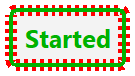
\includegraphics[scale=.2]{figs/maude-testStart}
}\qquad\qquad
\subcaptionbox{Rule \markInputR\label{fig:maude-markInput}}{
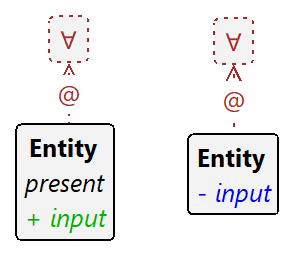
\includegraphics[scale=.2]{figs/maude-markInput}
}
\subcaptionbox{Condition \steadyR\label{fig:maude-steady}}{
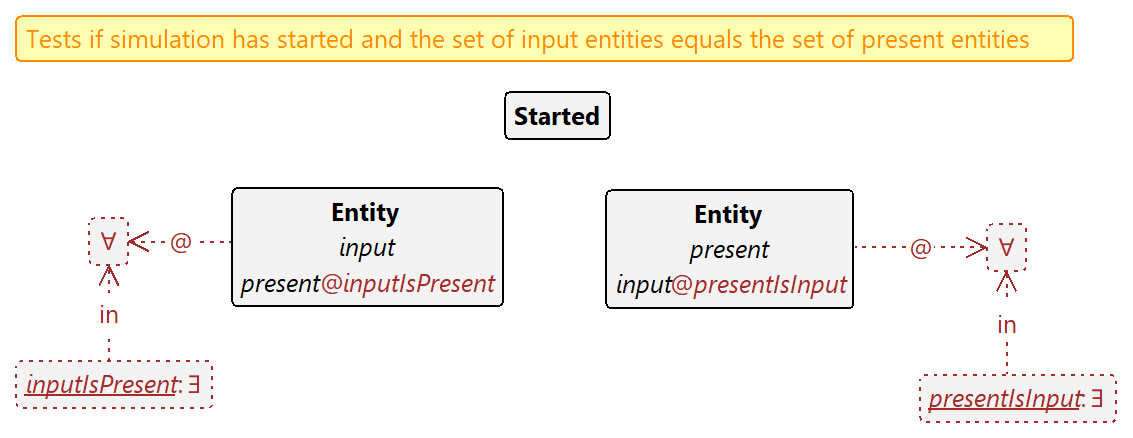
\includegraphics[scale=.2]{figs/maude-steady}
}
\caption{Additional rules and condition for detecting steadiness}
\label{fig:maude-mc}
\end{figure}

\begin{enumerate}
\item Given the context \verb=[k,ket]=, \GROOVE confirms the status of the following LTL properties:
\begin{itemize}
\item \verb=FG(steady -> akt)= is not satisfied; \GROOVE produces a counter-example.

\item \verb=G(erbb2 -> X(erbb2))= is satisfied.
\end{itemize}

\item Given the context \verb=[{e,egf,hrg}.korep]=, \GROOVE confirms the status of the following CTL properties:
\begin{itemize}
\item \verb=EF (steady & !akt)= is satisfied;
\item \verb=AF (steady & !akt)= is not satisfied.
\end{itemize}

\item Given the context \verb=[k,korept]=, \GROOVE confirms the status of the following LTL properties:
\begin{itemize}
\item \verb=G(pdk1 -> FG(steady -> akt))= is satisfied;
\item \verb=erbb1 R !pdk1= is satisfied.
\end{itemize}

\item Given the context \verb=[k,kge]=, \GROOVE confirms the status of the following CTL property:
\begin{itemize}
\item \verb=EG EF (steady -> !akt)= is satisfied. 
\end{itemize}
However, we want to point out that this property does not actually provide any useful guarantees, because the predicate \verb=steady= (both in \cite{DBLP:conf/cmsb/BallisBFO24} and in our encoding explained above) only tests for \emph{single-state} attractors. If the reaction system ends up in a multi-state loop, \verb=steady= will never be satisfied and hence the implication \verb=steady -> !akt= is \emph{always} satisfied, irregardless of whether or not \verb=akt= holds. Indeed, the state space of this scenario, visually reproduced in \Cref{fig:maude-gts}, has such a multi-state attractor (consisting of states \textit{s15} and \textit{s18}); in both of those states the predicate \verb=akt= holds, yet the state space as a whole satisfies the CTL property above.
\end{enumerate}
%
\begin{figure}\centering
\scalebox{.9}{% To use this figure in your LaTeX document
% import the package groove/resources/groove2tikz.sty
%
\begin{tikzpicture}[scale=.7,name prefix=rs-explore-gts-]
\node[start_node, active] (s0) {\ml{\uline{\textit{s0}}}};
\node[state_node] (s4) [right=.7 of s0] {\ml{\uline{\textit{s4}}\\\textit{erbb1}\\\textit{erbb2}\\\textit{erbb3}\\\textit{erk12}\\\textit{plcg}}};
\node[state_node] (s8) [right=.7 of s4] {\ml{\uline{\textit{s8}}\\\textit{akt}\\\textit{erk12}\\\textit{mek12}\\\textit{p70s6k}\\\textit{pdk1}\\\textit{pkca}\\\textit{plcg}}};
\node[state_node] (s11) [right=.7 of s8] {\ml{\uline{\textit{s11}}\\\textit{akt}\\\textit{erbb1}\\\textit{erbb2}\\\textit{erbb3}\\\textit{erk12}\\\textit{mek12}\\\textit{mtor}\\\textit{p70s6k}\\\textit{pdk1}\\\textit{pkca}\\\textit{plcg}}};
\node[state_node] (s15) [right=.7 of s11] {\ml{\uline{\textit{s15}}\\\textit{akt}\\\textit{erk12}\\\textit{mek12}\\\textit{mtor}\\\textit{p70s6k}\\\textit{pdk1}\\\textit{pkca}\\\textit{plcg}}};
\node[state_node] (s18) [right=.7 of s15] {\ml{\uline{\textit{s18}}\\\textit{akt}\\\textit{erbb1}\\\textit{erbb2}\\\textit{erbb3}\\\textit{erk12}\\\textit{mek12}\\\textit{mtor}\\\textit{p70s6k}\\\textit{pdk1}\\\textit{pkca}\\\textit{plcg}}};

\path[trans_edge](s0.east) -- node[lab] {\ml{fire}} (s4) ;
\path[trans_edge](s4.east) -- node[lab] {\ml{fire}} (s8) ;
\path[trans_edge](s8.east) -- node[lab] {\ml{fire}} (s11) ;
\path[trans_edge](s11.east) -- node[lab] {\ml{fire}} (s15) ;
\path[trans_edge](s15.15) -- node[lab] {\ml{fire}} (s18.165) ;
\path[trans_edge](s18.195) -- node[lab] {\ml{fire}} (s15.345) ;
\end{tikzpicture}
}
\caption{GTS for cancer scenario~4}
\label{fig:maude-gts}
\end{figure}
%
In replicating the results from \cite{DBLP:conf/cmsb/BallisBFO24}, we have had to make a few adjustments. The LTL formulas reported in \cite[Page~14]{DBLP:conf/cmsb/BallisBFO24} for scenarios 1 and~3 are actually \emph{not} literally the ones above, but use the predicate \verb=io-state= rather than \verb=isSteady=. We believe this to be erroneous, judging from the explanatory text, which is phrased in terms of steady states.\todo{A: Please check}

As a final observation, we note that the numbers of states in all these scenarios is actually quite small. We have already shown the 6-state scenario~4 in \Cref{fig:maude-gts}; the size of the others is given by the following table.
%
\begin{center}
\begin{tabular}{rlr}
\bf Nr. & \bf Context & \bf States \\
\hline\hline
1 & \tt [k,ket] & 4 \\
2 & \tt [{e,egf,hrg}.korep] & 10 \\
3 & \tt [k,korept] & 32 \\
4 & \tt [k,kge] & 6
\end{tabular}
\end{center}

